\section{Описание практической части}
\label{sec:Chapter4} \index{Chapter4}

% Если в рамках работы писался какой-то код, здесь должно быть его
% описание: выбранный язык и библиотеки и мотивы выбора, архитектура,
% схема функционирования, теоретическая сложность алгоритма, характеристики
% функционирования (скорость/память).

Согласно разработанной архитектуре, трассировщик и санитайзер представляют собой два отдельных процесса. Используя Unix-сокеты, санитайзер получает от трассировщика информацию о доступах к файлам и о порождении новых процессов, а от remake~--- дерево зависимостей и соответствие целей сборки номерам процессов (pid).

\begin{figure}[H]
    \centering
    \begin{tikzpicture}
    \node[style=draw, rounded corners, inner xsep=10pt, inner ysep=6pt] (sanitizer) at (-1, 0) {Санитайзер};
    \node[style=draw, rounded corners, inner xsep=10pt, inner ysep=6pt] (tracer) at (3.2, 0) {Трассировщик};
    \node[style=draw, rounded corners, inner xsep=10pt, inner ysep=6pt] (make) at (7, 0) {remake};
    \node[minimum width=2cm, minimum height=0.7cm, gray, style=draw, rounded corners] (child1) at (11, 1) {gcc};
    \node[minimum width=2cm, minimum height=0.7cm, gray, style=draw, rounded corners] (child2) at (11, 0) {mkdir};
    \node[minimum width=2cm, minimum height=0.7cm, gray, style=draw, rounded corners] (child3) at (11, -1) {...};

    \draw[dashed, line width=1pt, shorten >=2pt, shorten <=2pt, ->] (sanitizer) -- (tracer);
    \draw[dashed, line width=1pt, shorten >=2pt, shorten <=2pt, ->] (tracer) -- (make);
    \draw[dashed, line width=1pt, shorten >=2pt, shorten <=2pt, ->] (make) to[in=180, out=0] (child1);
    \draw[dashed, line width=1pt, shorten >=2pt, shorten <=2pt, ->] (make) to[in=180, out=0] (child2);
    \draw[dashed, line width=1pt, shorten >=2pt, shorten <=2pt, ->] (make) to[in=180, out=0] (child3);

    \draw[line width=1pt, shorten <=2pt] (10, 0.75) arc (90:180:0.5);
    \draw[line width=1pt, shorten <=2pt] (10, -0.25) arc (90:180:0.5);
    \draw[line width=1pt] (9.5, 0.25) -- (9.5, -0.75) arc (0:-90:0.5);
    \draw[line width=1pt] (7, -0.5) -- (7, -0.75) arc (0:-90:0.5);
    \draw[line width=1pt, shorten <=2pt, ->] (10, -1.25) -- (4, -1.25) arc (270:180:0.5) -- (3.5, -0.5);
    \node[font=\footnotesize] at (5.25, -1.0) {События ptrace};

    \draw[line width=1pt, shorten >=2pt, shorten <=2pt, ->] (4.5, 0.5) arc (0:90:0.5) -- (-1, 1.0) arc (90:180:0.5);
    \node[font=\footnotesize] at (1.8, 1.2) {События над файлами и процессами};

    \draw[line width=1pt, shorten >=2pt, shorten <=2pt, ->] (7.5, 0.5) -- (7.5, 1.0) arc (0:90:0.5) -- (-1.5, 1.5) arc (90:180:0.5) -- (-2.0, 0.5);
    \node[font=\footnotesize] at (3, 1.7) {Соответствие процессов целям и граф зависимостей};
\end{tikzpicture}
    \caption{Схема межпроцессного взаимодействия при сборке под санитайзером}
    \label{fig:parmasan-processes}
\end{figure}

Пунктирные стрелки на рис.~\ref{fig:parmasan-processes} связывают родительские процессы с дочерними.

Выбранная архитектура позволяет изолировать санитайзер от непосредственной работы с файловой системой и с дочерними процессами. Результат работы санитайзера определяется лишь сообщениями, которые он получает от трассировщика и от процессов remake. Позже это решение также позволит значительно ускорить итеративную отладку гонок.

Дерево зависимостей передаётся санитайзеру из Make-процесса. Это позволяет избежать написания своего синтаксического анализатора для Makefile. В дополнение, такой подход гарантирует, что граф зависимостей, на основании которого производится поиск гонок, в точности соответствует настоящему графу зависимостей, который используется самой утилитой Make.

Поскольку трассировщик является сравнительно тонкой обёрткой над системным вызовом \texttt{ptrace}, он был написан на языке Си. Для санитайзера, как для более сложного проекта, был выбран язык C\texttt{++}.

\subsection{Построение дерева процессов}
\label{subsec:pstree}

Информация о процессах приходит санитайзеру из двух источников. Первым трассировщик сообщает о создании нового процесса путём отслеживания системных вызовов \texttt{clone}, \texttt{spawn} и \texttt{fork}. Если процесс был порождён процессом remake, он должен передать информацию о цели, которой этот процесс соответствует. Это позволит санитайзеру соотнести операции над файлами с целями сборки (см.~\ref{subsubsec:link-ops-with-targets}).

По умолчанию трассировщик останавливает все новые процессы на первой инструкции. Это необходимо для того, чтобы успеть настроить перехват системных вызовов и передать санитайзеру информацию о созданном процессе раньше, чем тот начнёт совершать какие-либо действия. Когда санитайзер получает сообщение о создании нового процесса, он добавляет его в общее дерево и отправляет подтверждение трассировщику. Дождавшись ответа, трассировщик позволяет процессу начать работу.

Если процесс успеет открыть какой-то файл раньше, чем санитайзер узнает его цель, он не сможет отнести этот доступ к правильной цели, и может пропустить гонку. Поэтому цель, которой соответствует процесс, должна быть получена санитайзером раньше, чем этот процесс будет запущен. Это позволяет реализовать схема \texttt{fork/exec}. После вызова \texttt{fork} pid процесса становится известен. В этот момент remake отправляет его вместе с названием цели санитайзеру. Дождавшись ответного сообщения, и убедившись что санитайзер установил соответствие между процессом и целью, remake заканчивает создание нового процесса вызовом \texttt{exec}.

Утилита remake поддерживает несколько способов порождения новых процессов. Кроме классического \texttt{fork/exec} поддерживается и более эффективный метод, использующий \texttt{posix\_spawn}. Этот способ, однако, не позволяет узнать pid нового процесса перед его запуском. Его нужно отключить, указав флаг \texttt{-{}-disable-posix-spawn} в фазе configure.

Сообщая о гонке, санитайзер указывает два конфликтующих доступа, которые могут произойти в обратном порядке. Один из этих доступов может быть произведён процессом, который уже успел завершиться. В этом случае его pid может быть использован ядром повторно для другого процесса. В связи с этим для идентификации процессов в внутренних структурах санитайзера используется пара чисел (pid, эпоха). Каждый раз, когда pid используется повторно, эпоха инкрементируется. Это позволяет избежать конфликтов и однозначно ссылаться на уже завершённые процессы.

\subsection{Отслеживание операций над файлами}

\begin{table}[H]
    \centering
    \begin{tabular}{>{\raggedright\arraybackslash}m{4cm}>{\raggedright\arraybackslash}m{8cm}}
        \toprule
        \multicolumn{1}{c}{\textbf{Cистемный вызов}} & \multicolumn{1}{c}{\textbf{Cобытие для санитайзера}} \\
        \midrule
        \texttt{open(at)(at2)}                       & \texttt{read} или \texttt{write}                     \\
        \texttt{mkdir(at)}                           & \texttt{write}                                       \\
        \texttt{creat}                               & \texttt{write}                                       \\
        \texttt{rmdir}                               & \texttt{unlink}                                      \\
        \texttt{unlink(at)}                          & \texttt{unlink}                                      \\
        \texttt{rename(at)(at2)}                     & \texttt{unlink} целевого пути, если он существует.   \\
        \bottomrule
    \end{tabular}
    \caption{Системные вызовы над файлами, отслеживаемые трассировщиком}
    \label{tab:syscalls}
\end{table}

Трассировщик перехватывает операции над файлами и сообщает о них санитайзеру. На таблице~\ref{tab:syscalls} перечислены системные вызовы, соответствующие разным типам событий для санитайзера.

Флаги, переданные системному вызову \texttt{open}, могут указать, открывает ли процесс файл на чтение (\texttt{O\_RD}) или на запись (\texttt{O\_WR}). Если файл открыт на чтение и запись (\texttt{O\_RDWR}), трассировщик сообщает только о записи. Этого оказывается достаточно, поскольку ни в одном из рассматриваемых типов гонок чтение из файла не породит новых конфликтов.

Санитайзер работает в предположении, что если файл был открыт на чтение или запись, то процесс обязательно произведёт это чтение или запись. Это может быть верно не всегда: процесс может открыть файл в режиме \texttt{O\_RDWR}, и использовать полученный дескриптор только для чтения. Единственный способ избежать этой проблемы --- отслеживать системные вызовы \texttt{read} и \texttt{write}.

На практике такое решение оказывается неоправданным. На одном открытом файле \texttt{read} и \texttt{write} может быть вызван множество раз. Кроме операций над файлами, эти системные вызовы используются для работы с сокетами, вывода в консоль, чтения \texttt{signalfd}, и прочим. Перехват таких нагруженных системных вызовов многократно увеличивает объём обрабатываемых данных и замедляет работу санитайзера.

Поскольку санитайзер предполагает <<наихудший>> сценарий, подход с использованием флагов \texttt{open} не может привести к пропуску гонок, только к ложным срабатываниям. Несмотря на это, при тестировании санитайзера на реальных проектах таких случаев не было выявлено. Все утилиты gcc и стандартные утилиты Linux используют правильные флаги для \texttt{open}.

Переименование файла \textit{A} в \textit{B}, контринтуитивно, не эквивалентно удалению пути \textit{A} и созданию пути \textit{B}. При перемещении файла с помощью системного вызова \texttt{rename} его номер inode не изменяется. При этом, если путь назначения (\textit{B}) существовал, то inode, на которую он ссылался, теряет ссылку. Это эквивалентно удалению пути \textit{B}, а не \textit{A}. Cанитайзер учитывает переименование как удаление пути назначения. Это позволяет искать гонки на содержимом файла даже если он был переименован.

\subsection{Обработка вложенных Make}
\label{subsec:nested-make}

Крупные проекты бывают разделены на несколько схем сборки, каждая из которых отвечает за свой модуль. <<Корневой>> Makefile запускает их сборку, вызывая вложенные Make. Таким образом, проект можно представить как дерево из модулей. Гонки могут происходить между разными модулями одного проекта.

\begin{figure}[H]
    \centering
    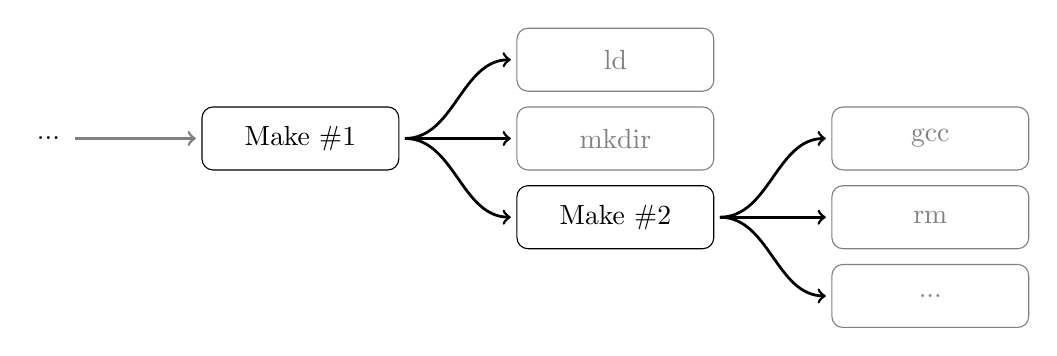
\begin{tikzpicture}
    \node (tracer) at (3.8, 0) {...};
    \node[minimum width=2.5cm, minimum height=0.8cm, style=draw, rounded corners] (make) at (7, 0) {Make~\#1};
    \node[minimum width=2.5cm, minimum height=0.8cm, gray, style=draw, rounded corners] (child1) at (11, 1) {ld};
    \node[minimum width=2.5cm, minimum height=0.8cm, gray, style=draw, rounded corners] (child2) at (11, 0) {mkdir};
    \node[minimum width=2.5cm, minimum height=0.8cm, style=draw, rounded corners] (child3) at (11, -1) {Make~\#2};

    \node[minimum width=2.5cm, minimum height=0.8cm, gray, style=draw, rounded corners] (child31) at (15, 0) {gcc};
    \node[minimum width=2.5cm, minimum height=0.8cm, gray, style=draw, rounded corners] (child32) at (15, -1) {rm};
    \node[minimum width=2.5cm, minimum height=0.8cm, gray, style=draw, rounded corners] (child33) at (15, -2) {...};

    \draw[gray, line width=1pt, shorten >=2pt, shorten <=2pt, ->] (tracer) -- (make);
    \draw[line width=1pt, shorten >=2pt, shorten <=2pt, ->] (make) to[in=180, out=0] (child1);
    \draw[line width=1pt, shorten >=2pt, shorten <=2pt, ->] (make) to[in=180, out=0] (child2);
    \draw[line width=1pt, shorten >=2pt, shorten <=2pt, ->] (make) to[in=180, out=0] (child3);

    \draw[line width=1pt, shorten >=2pt, shorten <=2pt, ->] (child3) to[in=180, out=0] (child31);
    \draw[line width=1pt, shorten >=2pt, shorten <=2pt, ->] (child3) to[in=180, out=0] (child32);
    \draw[line width=1pt, shorten >=2pt, shorten <=2pt, ->] (child3) to[in=180, out=0] (child33);

    % \node[gray, font=\small] (text1) at (6.7, -2) {События ptrace};
    % \node[gray, font=\small] (text1) at (1, -2) {События над файлами и процессами};
    % \node[gray, font=\small] (text2) at (3.5, 1.8) {Соответствие процессов целям и граф зависимостей};
\end{tikzpicture}
    \caption{Дерево процессов при использовании вложенных Make}
    \label{fig:nested-make-pstree}
\end{figure}

Рассмотрим процессы \texttt{gcc} и \texttt{ld} из рис.~\ref{fig:nested-make-pstree}. Предположим, что процесс \texttt{gcc} запускается в ходе сборки библиотеки \texttt{libfoo.a} одноимённой целью, \texttt{ld} --- целью \texttt{a.out} а Make~\#2 --- целью \texttt{libfoo}, как на рис.~\ref{fig:nested-make-pstree-2}.

\begin{figure}[H]
    \centering
    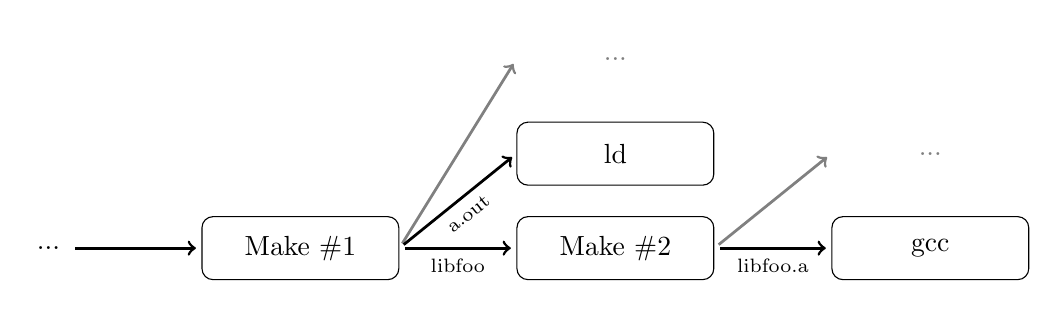
\begin{tikzpicture}
    \node (tracer) at (3.8, 0) {...};
    \node[minimum width=2.5cm, minimum height=0.8cm, style=draw, rounded corners] (make) at (7, 0) {Make~\#1};
    \node[minimum width=2.5cm, minimum height=0.8cm, gray] (child3) at (11, 2.4) {...};
    \node[minimum width=2.5cm, minimum height=0.8cm, style=draw, rounded corners] (child2) at (11, 1.2) {ld};
    \node[minimum width=2.5cm, minimum height=0.8cm, style=draw, rounded corners] (child1) at (11, 0) {Make~\#2};

    \node[minimum width=2.5cm, minimum height=0.8cm, gray] (child12) at (15, 1.2) {...};
    \node[minimum width=2.5cm, minimum height=0.8cm, style=draw, rounded corners] (child11) at (15, 0) {gcc};

    \draw[line width=1pt, shorten >=2pt, shorten <=2pt, ->] (tracer.east) -- (make.west);

    \draw[gray, line width=1pt, shorten >=2pt, shorten <=2pt, ->] (make.east) -- (child3.west);
    \draw[line width=1pt, shorten >=2pt, shorten <=2pt, ->] (make.east) -- (child2.west) node[font=\scriptsize, midway, sloped, below] {a.out};
    \draw[line width=1pt, shorten >=2pt, shorten <=2pt, ->] (make.east) -- (child1.west) node[font=\scriptsize, midway, sloped, below] {libfoo};

    \draw[gray, line width=1pt, shorten >=2pt, shorten <=2pt, ->] (child1.east) -- (child12.west);
    \draw[line width=1pt, shorten >=2pt, shorten <=2pt, ->] (child1.east) -- (child11.west) node[font=\scriptsize, midway, sloped, below] {libfoo.a};

    % \node[gray, font=\small] (text1) at (6.7, -2) {События ptrace};
    % \node[gray, font=\small] (text1) at (1, -2) {События над файлами и процессами};
    % \node[gray, font=\small] (text2) at (3.5, 1.8) {Соответствие процессов целям и граф зависимостей};
\end{tikzpicture}
    \caption{Дерево процессов с целями при использовании вложенных Make}
    \label{fig:nested-make-pstree-2}
\end{figure}

Предположим, что упомянутые процессы работают с одним и тем же файлом \texttt{libfoo.a}. Процесс \texttt{gcc} --- на запись, \texttt{ld} --- на чтение. Чтобы проверить наличие гонки, необходимо установить, есть ли зависимость между целями \texttt{libfoo.a} и \texttt{a.out}. Найти эту зависимость напрямую невозможно, поскольку эти цели принадлежат разным Makefile.

Как изображено на рис.~\ref{fig:nested-make-timeline}, цели вложенного Make-процесса выполняются в интервале времени работы внешней цели, породившей этот вложенный Make. Если между \texttt{libfoo} и \texttt{a.out} есть зависимость, это значит, что все цели вложенного Make (включая \texttt{libfoo.a}) закончат выполнение раньше, чем запустится \texttt{a.out}.

\begin{figure}[H]
    \centering
    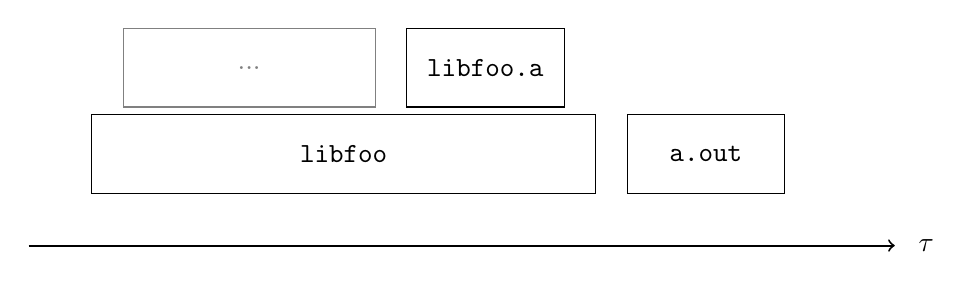
\begin{tikzpicture}
    \node[draw, minimum width=6.4cm, minimum height=1cm] at (4, 0) {\texttt{libfoo}};
    \node[draw, minimum width=2.0cm, minimum height=1cm] at (5.8, 1.1) {\texttt{libfoo.a}};
    \node[gray, draw, minimum width=3.2cm, minimum height=1cm] at (2.8, 1.1) {...};
    \node[draw, minimum width=2cm, minimum height=1cm] at (8.6, 0) {\texttt{a.out}};

%        \draw[dashed] (6.8, 1.6) -- (6.8, 3.0);
%        \draw[dashed] (7.2, 0.5) -- (7.2, 2.0);
%        \draw[dashed] (7.6, 0.5) -- (7.6, 1.0);

%        \node[font=\small, minimum width=6cm, text width=6cm] at (10, 3.0) {Завершение работы вложенной цели \texttt{libfoo.a}};
%        \node[font=\small, minimum width=6cm, text width=6cm] at (10.4, 2.0) {Завершение работы внешней цели \texttt{libfoo}};
%        \node[font=\small, minimum width=6cm, text width=6cm] at (10.8, 1.0) {Запуск целей, зависящих от \texttt{libfoo}};

    \node[font=\itshape] (time) at (11.4, -1.16) {$\tau$};
    \draw[line width=0.7pt, ->] (0, -1.16) to (11, -1.16);
\end{tikzpicture}
    \caption{Временная линия сборки при использовании вложенных Make}
    \label{fig:nested-make-timeline}
\end{figure}

В случае, если две цели из разных Makefile производят доступ к одному и тому же файлу, санитайзер <<поднимется>> на тот уровень, который породил обе этих цели, и будет производить поиск зависимости между соответствующими целями верхнего уровня. Этот <<подъём>> известен как задача поиска Lowest Common Ancestor (LCA). Она имеет несколько on-line решений:

\begin{enumerate}
    \item Линейный подъём, использующий глубину узлов дерева --- $O(n)$ в худшем случае.
    \item Двоичный подъём, требующий предварительного подсчёта ссылок на родителей уровней $2^i$ --- $O(\log{n})$ в худшем случае.
\end{enumerate}

Оба алгоритма имеют свои достоинства и недостатки. Линейный подъём дольше поднимается на большие расстояния, в то время как двоичный подъём требует предварительного подсчёта, что усложняет процедуру добавления новых процессов в дерево. Таким образом, оптимальный выбор алгоритма зависит от того, насколько часто санитайзеру придётся подниматься на большую высоту.

\subsubsection{Оценка средней дистанции подъёма}

Для выбора оптимального алгоритма был проведён эксперимент на нескольких проектах. Наибольшая средняя высота подъёма составила 0.74 при сборке gcc версии 13.1.0 для платформы x86-64 с флагом \texttt{-{}-disable-multilib}. Подробные результаты представлены на таб.~\ref{tab:ascend_distances}

\begin{table}[H]
    \centering
    \begin{tabular}{crD{.}{.}{-1}}
        \toprule
        Высота подъёма & Количество & \multicolumn{1}{l}{\% от общего числа} \\
        \midrule
        0              & 1270422    & 63.50\%                                \\
        1              & 314306     & 15.71\%                                \\
        2              & 176906     & 8.84\%                                 \\
        3              & 188222     & 9.40\%                                 \\
        4              & 34932      & 1.74\%                                 \\
        5              & 15562      & 0.77\%                                 \\
        6              & 260        & 0.0013\%                               \\
        \bottomrule
    \end{tabular}
    \caption{Количество подъёмов при сборке \texttt{gcc} версии 13.1.0}
    \label{tab:ascend_distances}
\end{table}

Среди проектов, выбранных для эксперимента, gcc является самым крупным. При сборке небольших проектов средняя высота подъёма меньше в сотни раз: на проекте Vim она составляет 0.004, а на strace --- 0.0028. Это указывает на то, что наиболее оптимальным алгоритмом будет метод линейного подъёма.

\subsection{Протокол взаимодействия}
\label{subsec:socket-protocol}

Архитектура инструмента предполагает обмен данными между процессами посредством сокета. Ниже представлен пример сообщения, которым трассировщик сообщает санитайзеру, что определённый процесс открыл файл в режиме чтения.

\begin{figure}[H]
    \centering
    \begin{tikzpicture}
    % symbol width = 10.2 / 47 = 0.217
    \node at (0, 0) {\texttt{ASYNC READ 16 /lib64/libc.so.6 1005 15 646356 7}};

    % ASYNC:
    % -5.1 + 0.217 * 0 = -5.1
    % -5.1 + 0.217 * 5 = -4.015
    \draw[line width=0.7pt] (-5.1, -0.25) -- (-4.0375, -0.25);
    \draw[line width=0.7pt] (-5.1, -0.25) -- (-5.1, -4.5);
    \node[align=flush left, font=\footnotesize, minimum width=4cm, text width=4cm] at (-3.2, -5.1) {Флаг синхронности сообщения.};


    % READ:
    % -5.1 + 0.217 * 6 = -3.798
    % -5.1 + 0.217 * 10 = -2.93
    \draw[line width=0.7pt] (-3.798, -0.25) -- (-2.93, -0.25);
    \draw[line width=0.7pt] (-3.798, -0.25) -- (-3.798, -3);
    \node[align=flush left, font=\footnotesize, minimum width=5cm, text width=5cm] at (-1.398, -3.8) {Название события. В данном случае~--- \texttt{READ}~--- чтение файла.};

    % 16:
    % -5.1 + 0.217 * 11 = -2.713
    % -5.1 + 0.217 * 13 = -2.279
    \draw[line width=0.7pt] (-2.713, -0.25) -- (-2.279, -0.25);
    \draw[line width=0.7pt] (-2.713, -0.25) -- (-2.713, -2);
    \node[align=flush left, font=\footnotesize, minimum width=4cm, text width=4cm] at (-0.813, -2.6) {Длина строки, следующей далее.};

    % /lib64/libc.so.6:
    % -5.1 + 0.217 * 14 = -2.062
    % -5.1 + 0.217 * 30 = 1.41
    \draw[line width=0.7pt] (-2.062, -0.25) -- (1.41, -0.25);
    \draw[line width=0.7pt] (-2.062, -0.25) -- (-2.062, -0.5);
    \node[align=flush left, font=\footnotesize, minimum width=3cm, text width=3cm] at (-0.662, -1.3) {Путь, по которому процесс обратился к файлу.};

    % 1005:
    % -5.1 + 0.217 * 31 = 1.627
    % -5.1 + 0.217 * 35 = 2.495
    \draw[line width=0.7pt] (1.627, -0.25) -- (2.495, -0.25);
    \draw[line width=0.7pt] (1.627, -0.25) -- (1.627, -4);
    \node[align=flush left, font=\footnotesize, minimum width=6cm, text width=6cm] at (4.527, -4.6) {pid процесса, производящего доступ к файлу.};

    % 15:
    % -5.1 + 0.217 * 36 = 2.712
    % -5.1 + 0.217 * 38 = 3.146
    \draw[line width=0.7pt] (2.712, -0.25) -- (3.146, -0.25);
    \draw[line width=0.7pt] (2.712, -0.25) -- (2.712, -3);
    \node[align=flush left, font=\footnotesize, minimum width=4cm, text width=4cm] at (4.612, -3.6) {Device number файловой системы.};

    % 646356:
    % -5.1 + 0.217 * 39 = 3.363
    % -5.1 + 0.217 * 45 = 4.665
    \draw[line width=0.7pt] (3.363, -0.25) -- (4.665, -0.25);
    \draw[line width=0.7pt] (3.363, -0.25) -- (3.363, -2);
    \node[align=flush left, font=\footnotesize, minimum width=4cm, text width=4cm] at (5.263, -2.6) {Номер inode прочитанного файла.};

    % 7:
    % -5.1 + 0.217 * 46 = 4.882
    % -5.1 + 0.217 * 47 = 5.099
    \draw[line width=0.7pt] (4.882, -0.25) -- (5.099, -0.25);
    \draw[line width=0.7pt] (4.882, -0.25) -- (4.882, -0.5);
    \node[align=flush left, font=\footnotesize, minimum width=3cm, text width=3cm] at (6.282, -1.3) {Код возврата системного вызова \texttt{open}.};
\end{tikzpicture}
    \caption{Пример сообщения, передаваемого санитайзеру трассировщиком}
    \label{fig:parmasan-message-example}
\end{figure}

Любое сообщение, отправляемое санитайзеру, должно начинаться с флага синхронности (слова \texttt{SYNC} или \texttt{ASYNC}). Он указывает, ожидает ли отправляющая сторона ответное сообщение, как подтверждение того что событие было обработано. Пункт~\ref{subsec:pstree} содержит примеры некоторых типов сообщений, требующих подобной синхронизации.

Следующее слово определяет тип передаваемого события. Каждый тип имеет свой набор аргументов. Если аргументом является строка (например, путь к файлу), то перед её началом передаётся её длина и один разделяющий символ пробела. Такой простой формат упрощает составление и разбор сообщений до нескольких вызовов \texttt{memcpy} и \texttt{sprintf} / \texttt{sscanf}.

Перечень сообщений, отправляемых трассировщиком санитайзеру:

\begin{enumerate}
    \item \texttt{INIT TRACER}~--- инициализирующее сообщение.
    \item \texttt{CHILD <pid> <ppid> <cmdline>}~--- Сообщает о создании нового процесса в дереве, или о том, что существующий процесс сменил свою \texttt{cmdline}, вызвав \texttt{exec}. Это сообщение всегда является синхронным, см.~\ref{subsec:pstree}.
    \item \texttt{READ <path> <pid> <devnum> <inum> <}код возврата\texttt{>}~--- событие открытия процессом файла на чтение.
    \item \texttt{WRITE <path> <pid> <devnum> <inum> <}код возврата\texttt{>}
    ~--- событие открытия процессом файла на запись.
    \item \texttt{UNLINK <path> <pid> <devnum> <inum> <}код возврата\texttt{>}~--- событие удаления пути (directory entry)
    \item \texttt{INODE\_UNLINK <path> <pid> <devnum> <inum> <}код возврата\texttt{>}~--- дублирует сообщение \texttt{UNLINK} в случае, если удалённый путь был последней жёсткой ссылкой на свою inode.
    \item \texttt{DIE <pid>}~--- сообщает о завершении работы процесса с указанным pid. Если свою работу завершает сам трассировщик, он отправляет это сообщение с собственным pid. В этом случае сообщение должно быть синхронным. Это будет гарантировать, что санитайзер успеет обработать все предыдущие сообщения от трассировщика прежде, чем получит сигнал \texttt{SIGCHLD} и остановится.
\end{enumerate}

Перечень сообщений, отправляемых процессом remake санитайзеру:

\begin{enumerate}
    \item \texttt{INIT MAKE}~--- инициализирующее сообщение.
    \item \texttt{TARGET\_PID <pid> <ppid> <cmdline>}~--- Устанавливает соответствие между процессом с указанным pid и целью, породившей его. Это сообщение всегда является синхронным, см.~\ref{subsec:pstree}.
    \item \texttt{DEPENDENCY <target\_a> <target\_b>}~--- Сообщает о наличии зависимости между двумя целями. Это сообщение должно являться синхронным, поскольку санитайзер должен получить весь граф зависимостей, прежде чем сможет находить потенциальные гонки между получаемыми им доступами.
\end{enumerate}

В обратную сторону санитайзер может отправить только слово \texttt{ACK} (от англ.~--- Acknowledged, принято). Оно отправляется как подтверждение завершения обработки предыдущего сообщения, если это требуется флагом синхронности.

Санитайзер должен знать, какой pid имеет отправитель каждого сообщения. Ядро Linux позволяет получить эти данные, используя системный вызов \texttt{getsockopt} и флаг \texttt{SO\_PEERCRED} (см.~\cite{unix-sockets}). Это избавляет от необходимости передавать эти данные по сокету.

В качестве режима для сокета был выбран \texttt{SOCK\_SEQPACKET}. Он гарантирует порядок доставки и сохранение границ сообщений (см. пункт 2.10.6 в стандарте POSIX~\cite{8277153}).

Имена событий подобраны таким образом, чтобы их можно было отличать по первому символу (сообщение \texttt{INIT} является исключением, но его отличает то, что оно всегда идёт первым). Это позволяет использовать \texttt{switch} для вызова нужного обработчика. Несмотря на то, что передаваемые сообщения являются человекочитаемыми, а не бинарными, простота протокола позволяет избежать значительных потерь в производительности.

\subsection{Режим интерактивной отладки}
\label{subsec:interactive-debug}

При отладке состояний гонок разработчикам часто требуется многократно пересобирать проект, устанавливая отладочные выводы на сборке определённых целей. Разработанный инструмент предлагает несколько функций, упрощающих этот процесс:

\begin{enumerate}
    \item Точки останова. Санитайзер позволяет приостанавливать сборку на определённых действиях с файлами или при обнаружении гонки. При срабатывании точки останова санитайзер предоставляет пользователю интерактивную консоль, с помощью которой можно вывести информацию о текущем состоянии сборки, а именно:

    \begin{itemize}
        \item Цель, при сборке которой произошел последний доступ к файлу;
        \item Процесс, который произвёл этот доступ;
        \item Информацию по любому процессу, даже завершённому:
        \begin{itemize}
            \item Командную строку процесса;
            \item Список целей его Makefile, если он является Make-процессом;
            \item Цепочку его родительских процессов;
            \item Поддерево процессов, порожденных им.
        \end{itemize}
    \end{itemize}

    Интерактивная консоль избавляет разработчика от необходимости искать эти данные в Makefile.

    \item Быстрое воспроизведение записи сборки. Если перенаправить в файл все сообщения, поступающие санитайзеру, и передать их на вход повторно, то результат его работы будет таким же, как и во время настоящей сборки.

    \begin{figure}[H]
        \centering
        \begin{tikzpicture}
    \node[style=draw, rounded corners, inner xsep=10pt, inner ysep=6pt] (parmasan) at (5, -2.5) {Санитайзер в режиме чтения лога};
    \node[style=draw, rounded corners, inner xsep=10pt, inner ysep=6pt] (trace) at (-1, -2.5) {Лог};
    \node[style=draw, rounded corners, minimum width=3cm, inner ysep=6pt] (logger) at (-1, 0) {Логгер};
    \node[gray, style=draw, rounded corners, inner xsep=10pt, inner ysep=6pt] (tracer) at (3.2, 0) {Трассировщик};
    \node[gray, style=draw, rounded corners, inner xsep=10pt, inner ysep=6pt] (make) at (7, 0) {remake*};
    \node[minimum width=2cm, minimum height=0.7cm, gray, style=draw, rounded corners] (child1) at (11, 1) {gcc};
    \node[minimum width=2cm, minimum height=0.7cm, gray, style=draw, rounded corners] (child2) at (11, 0) {mkdir};
    \node[minimum width=2cm, minimum height=0.7cm, gray, style=draw, rounded corners] (child3) at (11, -1) {...};

    \draw[dashed, gray, line width=1pt, shorten >=2pt, shorten <=2pt, ->] (logger) -- (tracer);
    \draw[dashed, gray, line width=1pt, shorten >=2pt, shorten <=2pt, ->] (tracer) -- (make);
    \draw[dashed, gray, line width=1pt, shorten >=2pt, shorten <=2pt, ->] (make) to[in=180, out=0] (child1);
    \draw[dashed, gray, line width=1pt, shorten >=2pt, shorten <=2pt, ->] (make) to[in=180, out=0] (child2);
    \draw[dashed, gray, line width=1pt, shorten >=2pt, shorten <=2pt, ->] (make) to[in=180, out=0] (child3);

    \draw[gray, line width=1pt, shorten <=2pt] (10, 0.75) arc (90:180:0.5);
    \draw[gray, line width=1pt, shorten <=2pt] (10, -0.25) arc (90:180:0.5);
    \draw[gray, line width=1pt] (9.5, 0.25) -- (9.5, -0.75) arc (0:-90:0.5);
    \draw[gray, line width=1pt] (7, -0.5) -- (7, -0.75) arc (0:-90:0.5);
    \draw[gray, line width=1pt, shorten <=2pt, ->] (10, -1.25) -- (4, -1.25) arc (270:180:0.5) -- (3.5, -0.5);
    \node[gray, font=\small] at (5.25, -1.0) {События ptrace};

    \draw[gray, line width=1pt, shorten >=2pt, shorten <=2pt, ->] (4.5, 0.5) arc (0:90:0.5) -- (-1, 1.0) arc (90:180:0.5);
    \node[gray, font=\small] at (1.8, 1.2) {События над файлами и процессами};

    \draw[gray, line width=1pt, shorten >=2pt, shorten <=2pt, ->] (7.5, 0.5) -- (7.5, 1.0) arc (0:90:0.5) -- (-1.5, 1.5) arc (90:180:0.5) -- (-2.0, 0.5);
    \node[gray, font=\small] at (3, 1.7) {Соответствие процессов целям и граф зависимостей};

    \draw[line width=1pt, shorten >=2pt, shorten <=2pt, ->] (trace) -- (parmasan);
    \draw[line width=1pt, shorten >=2pt, shorten <=2pt, ->] (logger) -- (trace);
\end{tikzpicture}
        \caption{Запись и воспроизведение лога сборки}
        \label{fig:build-dumping}
    \end{figure}

    Такое <<воспроизведение>> быстрее обычной пересборки проекта. Чтение записи сборки gcc 13.1.0 занимает у санитайзера 70 секунд, в то время как пересборка проекта с использованием восьми потоков занимает 50 минут.

    В сочетании с предыдущим пунктом эта функция позволяет производить итеративную отладку. После изменения точек останова, разработчик может быстро перезапустить запись, и не ждать полной пересборки.

    В случае, если санитайзер читает лог сборки, а не получает сообщения из сокета, использовать \texttt{SO\_PEERCRED} для получения pid отправителя невозможно. Эти данные указываются в логе явно, в начале каждого сообщения.
\end{enumerate}

Для реализации точек останова в санитайзер был добавлен отладочный режим. При его активации, все передаваемые по сокету сообщения становятся синхронными. При срабатывании точки останова на определённом доступе к файлу санитайзер перестаёт отправлять \texttt{ACK}-сообщения. Это приводит к тому, что трассировщик не позволяет процессам продолжить работу, и останавливает сборку.

Точка останова может быть привязана к произвольному множеству путей, задаваемым одним или несколькими glob--выражениями. Санитайзер конвертирует их в МПДКА, поэтому сложность проверки не растёт с увеличением количества точек останова. Санитайзер может добавить к существующему автомату новый, отвечающий за срабатывание на новой точке останова, с использованием логического <<ИЛИ>>. Затем сумму этих автоматов можно привести к новому МПДКА. Это позволяет добавлять и удалять точки останова в любой момент отладки без ухудшения производительности (удаление точки останова эквивалентно добавлению инвертированного автомата c логическим <<И>>).

\subsection{Тестирование и сравнение}
\label{subsec:testing}

По мере разработки проекта был разработан набор из 23 автоматических тестов, проверяющих поведение санитайзера в известных крайних случаях. Среди них:

\begin{itemize}
    \item Обнаружение гонок, включающих:
    \begin{itemize}
        \item Обновление Makefile, влекущее перезапуск Make;
        \item Доступы, производимые самим Make-процессом.
        \item Создание вложенных директорий;
        \item Указание более чем одной цели для сборки Make-процессом;
        \item Использование шаблонных правил;
        \item Запуск вложенных Make.
    \end{itemize}
    \item Разрешение символических ссылок при доступе к файлу, но игнорирование их при удалении;
    \item Корректная нормализация пути (удаление \texttt{.} и \texttt{..});
\end{itemize}

Тестирование производится автоматически с использованием CI на LXC-контейнерах с тремя разными системами:

\begin{itemize}
    \item Ubuntu Mantic;
    \item OpenRC Gentoo 6.8.1;
    \item Alpine 3.19.
\end{itemize}

Сергей Трофимович, разработчик режима Make \texttt{-{}-shuffle}, опубликовал в своём блоге список проектов, в которых ему удалось обнаружить гонки с использованием этого режима~\cite{trofi-make-shuffle}. Оценка эффективности разработанного санитайзера производилась путём запуска его на проектах из этого же списка и сравнении полученных гонок с перечнем известных, обнаруженных ранее.

\begin{figure}[H]
    \centering
    \begin{tikzpicture}[gnuplot]
%% generated with GNUPLOT 6.0p0 (Lua 5.4; terminal rev. Jun 2020, script rev. 118)
%% Thu Jun 13 15:54:13 2024
\path (0.000,0.000) rectangle (14.000,8.000);
\gpcolor{color=gp lt color border}
\gpsetlinetype{gp lt border}
\gpsetdashtype{gp dt solid}
\gpsetlinewidth{1.00}
\draw[gp path] (0.828,0.368)--(1.008,0.368);
\draw[gp path] (13.447,0.368)--(13.267,0.368);
\node[gp node right] at (0.644,0.368) {$-2$};
\draw[gp path] (0.828,1.495)--(1.008,1.495);
\draw[gp path] (13.447,1.495)--(13.267,1.495);
\node[gp node right] at (0.644,1.495) {$0$};
\draw[gp path] (0.828,2.621)--(1.008,2.621);
\draw[gp path] (13.447,2.621)--(13.267,2.621);
\node[gp node right] at (0.644,2.621) {$2$};
\draw[gp path] (0.828,3.748)--(1.008,3.748);
\draw[gp path] (13.447,3.748)--(13.267,3.748);
\node[gp node right] at (0.644,3.748) {$4$};
\draw[gp path] (0.828,4.874)--(1.008,4.874);
\draw[gp path] (13.447,4.874)--(13.267,4.874);
\node[gp node right] at (0.644,4.874) {$6$};
\draw[gp path] (0.828,6.001)--(1.008,6.001);
\draw[gp path] (13.447,6.001)--(13.267,6.001);
\node[gp node right] at (0.644,6.001) {$8$};
\draw[gp path] (0.828,7.128)--(1.008,7.128);
\draw[gp path] (13.447,7.128)--(13.267,7.128);
\node[gp node right] at (0.644,7.128) {$10$};
\node[gp node left,rotate=50.0,font={\fontsize{8.0pt}{9.6pt}\selectfont}] at (1.543,4.424) {ocamlbuild};
\node[gp node left,rotate=50.0,font={\fontsize{8.0pt}{9.6pt}\selectfont}] at (1.964,4.424) {Groff};
\node[gp node left,rotate=50.0,font={\fontsize{8.0pt}{9.6pt}\selectfont}] at (2.384,4.424) {GCC};
\node[gp node left,rotate=50.0,font={\fontsize{8.0pt}{9.6pt}\selectfont}] at (2.805,3.861) {slang};
\node[gp node left,rotate=50.0,font={\fontsize{8.0pt}{9.6pt}\selectfont}] at (3.226,3.861) {C/Migemo};
\node[gp node left,rotate=50.0,font={\fontsize{8.0pt}{9.6pt}\selectfont}] at (3.646,3.297) {subversion};
\node[gp node left,rotate=50.0,font={\fontsize{8.0pt}{9.6pt}\selectfont}] at (4.067,3.297) {Vim};
\node[gp node left,rotate=50.0,font={\fontsize{8.0pt}{9.6pt}\selectfont}] at (4.488,3.297) {Notion};
\node[gp node left,rotate=50.0,font={\fontsize{8.0pt}{9.6pt}\selectfont}] at (4.908,3.297) {Heimdal};
\node[gp node left,rotate=50.0,font={\fontsize{8.0pt}{9.6pt}\selectfont}] at (5.329,3.297) {GPM};
\node[gp node left,rotate=50.0,font={\fontsize{8.0pt}{9.6pt}\selectfont}] at (5.749,3.297) {GHC};
\node[gp node left,rotate=50.0,font={\fontsize{8.0pt}{9.6pt}\selectfont}] at (6.170,2.734) {libplist};
\node[gp node left,rotate=50.0,font={\fontsize{8.0pt}{9.6pt}\selectfont}] at (6.591,2.734) {jhead};
\node[gp node left,rotate=50.0,font={\fontsize{8.0pt}{9.6pt}\selectfont}] at (7.011,2.734) {bitlbee-facebook};
\node[gp node left,rotate=50.0,font={\fontsize{8.0pt}{9.6pt}\selectfont}] at (7.432,2.734) {OpenIPMI};
\node[gp node left,rotate=50.0,font={\fontsize{8.0pt}{9.6pt}\selectfont}] at (7.853,2.734) {Ispell};
\node[gp node left,rotate=50.0,font={\fontsize{8.0pt}{9.6pt}\selectfont}] at (8.273,2.734) {GNU-EFI};
\node[gp node left,rotate=50.0,font={\fontsize{8.0pt}{9.6pt}\selectfont}] at (8.694,2.734) {Angsd};
\node[gp node left,rotate=50.0,font={\fontsize{8.0pt}{9.6pt}\selectfont}] at (9.114,2.171) {x264};
\node[gp node left,rotate=50.0,font={\fontsize{8.0pt}{9.6pt}\selectfont}] at (9.535,2.171) {strace};
\node[gp node left,rotate=50.0,font={\fontsize{8.0pt}{9.6pt}\selectfont}] at (9.956,2.171) {ski};
\node[gp node left,rotate=50.0,font={\fontsize{8.0pt}{9.6pt}\selectfont}] at (10.376,2.171) {liburing};
\node[gp node left,rotate=50.0,font={\fontsize{8.0pt}{9.6pt}\selectfont}] at (10.797,2.171) {exifprobe};
\node[gp node left,rotate=50.0,font={\fontsize{8.0pt}{9.6pt}\selectfont}] at (11.218,2.171) {efivar};
\node[gp node left,rotate=50.0,font={\fontsize{8.0pt}{9.6pt}\selectfont}] at (11.638,2.171) {blahtexml};
\node[gp node left,rotate=50.0,font={\fontsize{8.0pt}{9.6pt}\selectfont}] at (12.059,2.171) {avldrums.lv2};
\node[gp node left,rotate=50.0,font={\fontsize{8.0pt}{9.6pt}\selectfont}] at (12.480,2.171) {Src-Highlite};
\node[gp node left,rotate=50.0,font={\fontsize{8.0pt}{9.6pt}\selectfont}] at (12.900,1.607) {ldns};
\node[gp node left,font={\fontsize{8.0pt}{9.6pt}\selectfont}] at (1.669,6.846) {MinGW-w64};
\node[gp node right,font={\fontsize{8.0pt}{9.6pt}\selectfont}] at (12.054,7.326) {Гонки, обнаруженные обоими инструментами};
\def\gpfillpath{(12.201,7.265)--(13.116,7.265)--(13.116,7.388)--(12.201,7.388)--cycle}
\gpfill{color=gpbgfillcolor} \gpfillpath;
\gpfill{rgb color={0.000,0.000,0.000},gp pattern 3,pattern color=.} \gpfillpath;
\gpcolor{rgb color={0.000,0.000,0.000}}
\gpsetlinewidth{2.00}
\draw[gp path] (12.201,7.265)--(13.116,7.265)--(13.116,7.387)--(12.201,7.387)--cycle;
\def\gpfillpath{(1.059,1.495)--(1.439,1.495)--(1.439,4.312)--(1.059,4.312)--cycle}
\gpfill{color=gpbgfillcolor} \gpfillpath;
\gpfill{rgb color={0.000,0.000,0.000},gp pattern 3,pattern color=.} \gpfillpath;
\draw[gp path] (1.059,1.495)--(1.059,4.311)--(1.438,4.311)--(1.438,1.495)--cycle;
\def\gpfillpath{(1.480,1.495)--(1.860,1.495)--(1.860,2.622)--(1.480,2.622)--cycle}
\gpfill{color=gpbgfillcolor} \gpfillpath;
\gpfill{rgb color={0.000,0.000,0.000},gp pattern 3,pattern color=.} \gpfillpath;
\draw[gp path] (1.480,1.495)--(1.480,2.621)--(1.859,2.621)--(1.859,1.495)--cycle;
\def\gpfillpath{(1.901,1.495)--(2.280,1.495)--(2.280,2.059)--(1.901,2.059)--cycle}
\gpfill{color=gpbgfillcolor} \gpfillpath;
\gpfill{rgb color={0.000,0.000,0.000},gp pattern 3,pattern color=.} \gpfillpath;
\draw[gp path] (1.901,1.495)--(1.901,2.058)--(2.279,2.058)--(2.279,1.495)--cycle;
\def\gpfillpath{(2.321,1.495)--(2.701,1.495)--(2.701,1.496)--(2.321,1.496)--cycle}
\gpfill{color=gpbgfillcolor} \gpfillpath;
\gpfill{rgb color={0.000,0.000,0.000},gp pattern 3,pattern color=.} \gpfillpath;
\draw[gp path] (2.321,1.495)--(2.700,1.495)--cycle;
\def\gpfillpath{(2.742,1.495)--(3.121,1.495)--(3.121,3.186)--(2.742,3.186)--cycle}
\gpfill{color=gpbgfillcolor} \gpfillpath;
\gpfill{rgb color={0.000,0.000,0.000},gp pattern 3,pattern color=.} \gpfillpath;
\draw[gp path] (2.742,1.495)--(2.742,3.185)--(3.120,3.185)--(3.120,1.495)--cycle;
\def\gpfillpath{(3.163,1.495)--(3.542,1.495)--(3.542,3.186)--(3.163,3.186)--cycle}
\gpfill{color=gpbgfillcolor} \gpfillpath;
\gpfill{rgb color={0.000,0.000,0.000},gp pattern 3,pattern color=.} \gpfillpath;
\draw[gp path] (3.163,1.495)--(3.163,3.185)--(3.541,3.185)--(3.541,1.495)--cycle;
\def\gpfillpath{(3.583,1.495)--(3.963,1.495)--(3.963,2.059)--(3.583,2.059)--cycle}
\gpfill{color=gpbgfillcolor} \gpfillpath;
\gpfill{rgb color={0.000,0.000,0.000},gp pattern 3,pattern color=.} \gpfillpath;
\draw[gp path] (3.583,1.495)--(3.583,2.058)--(3.962,2.058)--(3.962,1.495)--cycle;
\def\gpfillpath{(4.004,1.495)--(4.383,1.495)--(4.383,2.059)--(4.004,2.059)--cycle}
\gpfill{color=gpbgfillcolor} \gpfillpath;
\gpfill{rgb color={0.000,0.000,0.000},gp pattern 3,pattern color=.} \gpfillpath;
\draw[gp path] (4.004,1.495)--(4.004,2.058)--(4.382,2.058)--(4.382,1.495)--cycle;
\def\gpfillpath{(4.424,1.495)--(4.804,1.495)--(4.804,2.622)--(4.424,2.622)--cycle}
\gpfill{color=gpbgfillcolor} \gpfillpath;
\gpfill{rgb color={0.000,0.000,0.000},gp pattern 3,pattern color=.} \gpfillpath;
\draw[gp path] (4.424,1.495)--(4.424,2.621)--(4.803,2.621)--(4.803,1.495)--cycle;
\def\gpfillpath{(4.845,1.495)--(5.225,1.495)--(5.225,2.622)--(4.845,2.622)--cycle}
\gpfill{color=gpbgfillcolor} \gpfillpath;
\gpfill{rgb color={0.000,0.000,0.000},gp pattern 3,pattern color=.} \gpfillpath;
\draw[gp path] (4.845,1.495)--(4.845,2.621)--(5.224,2.621)--(5.224,1.495)--cycle;
\def\gpfillpath{(5.266,1.495)--(5.645,1.495)--(5.645,2.059)--(5.266,2.059)--cycle}
\gpfill{color=gpbgfillcolor} \gpfillpath;
\gpfill{rgb color={0.000,0.000,0.000},gp pattern 3,pattern color=.} \gpfillpath;
\draw[gp path] (5.266,1.495)--(5.266,2.058)--(5.644,2.058)--(5.644,1.495)--cycle;
\def\gpfillpath{(5.686,1.495)--(6.066,1.495)--(6.066,2.059)--(5.686,2.059)--cycle}
\gpfill{color=gpbgfillcolor} \gpfillpath;
\gpfill{rgb color={0.000,0.000,0.000},gp pattern 3,pattern color=.} \gpfillpath;
\draw[gp path] (5.686,1.495)--(5.686,2.058)--(6.065,2.058)--(6.065,1.495)--cycle;
\def\gpfillpath{(6.107,1.495)--(6.487,1.495)--(6.487,2.059)--(6.107,2.059)--cycle}
\gpfill{color=gpbgfillcolor} \gpfillpath;
\gpfill{rgb color={0.000,0.000,0.000},gp pattern 3,pattern color=.} \gpfillpath;
\draw[gp path] (6.107,1.495)--(6.107,2.058)--(6.486,2.058)--(6.486,1.495)--cycle;
\def\gpfillpath{(6.528,1.495)--(6.907,1.495)--(6.907,2.059)--(6.528,2.059)--cycle}
\gpfill{color=gpbgfillcolor} \gpfillpath;
\gpfill{rgb color={0.000,0.000,0.000},gp pattern 3,pattern color=.} \gpfillpath;
\draw[gp path] (6.528,1.495)--(6.528,2.058)--(6.906,2.058)--(6.906,1.495)--cycle;
\def\gpfillpath{(6.948,1.495)--(7.328,1.495)--(7.328,2.059)--(6.948,2.059)--cycle}
\gpfill{color=gpbgfillcolor} \gpfillpath;
\gpfill{rgb color={0.000,0.000,0.000},gp pattern 3,pattern color=.} \gpfillpath;
\draw[gp path] (6.948,1.495)--(6.948,2.058)--(7.327,2.058)--(7.327,1.495)--cycle;
\def\gpfillpath{(7.369,1.495)--(7.748,1.495)--(7.748,1.496)--(7.369,1.496)--cycle}
\gpfill{color=gpbgfillcolor} \gpfillpath;
\gpfill{rgb color={0.000,0.000,0.000},gp pattern 3,pattern color=.} \gpfillpath;
\draw[gp path] (7.369,1.495)--(7.747,1.495)--cycle;
\def\gpfillpath{(7.789,1.495)--(8.169,1.495)--(8.169,1.496)--(7.789,1.496)--cycle}
\gpfill{color=gpbgfillcolor} \gpfillpath;
\gpfill{rgb color={0.000,0.000,0.000},gp pattern 3,pattern color=.} \gpfillpath;
\draw[gp path] (7.789,1.495)--(8.168,1.495)--cycle;
\def\gpfillpath{(8.210,1.495)--(8.590,1.495)--(8.590,2.059)--(8.210,2.059)--cycle}
\gpfill{color=gpbgfillcolor} \gpfillpath;
\gpfill{rgb color={0.000,0.000,0.000},gp pattern 3,pattern color=.} \gpfillpath;
\draw[gp path] (8.210,1.495)--(8.210,2.058)--(8.589,2.058)--(8.589,1.495)--cycle;
\def\gpfillpath{(8.631,1.495)--(9.010,1.495)--(9.010,2.059)--(8.631,2.059)--cycle}
\gpfill{color=gpbgfillcolor} \gpfillpath;
\gpfill{rgb color={0.000,0.000,0.000},gp pattern 3,pattern color=.} \gpfillpath;
\draw[gp path] (8.631,1.495)--(8.631,2.058)--(9.009,2.058)--(9.009,1.495)--cycle;
\def\gpfillpath{(9.051,1.495)--(9.431,1.495)--(9.431,2.059)--(9.051,2.059)--cycle}
\gpfill{color=gpbgfillcolor} \gpfillpath;
\gpfill{rgb color={0.000,0.000,0.000},gp pattern 3,pattern color=.} \gpfillpath;
\draw[gp path] (9.051,1.495)--(9.051,2.058)--(9.430,2.058)--(9.430,1.495)--cycle;
\def\gpfillpath{(9.472,1.495)--(9.852,1.495)--(9.852,2.059)--(9.472,2.059)--cycle}
\gpfill{color=gpbgfillcolor} \gpfillpath;
\gpfill{rgb color={0.000,0.000,0.000},gp pattern 3,pattern color=.} \gpfillpath;
\draw[gp path] (9.472,1.495)--(9.472,2.058)--(9.851,2.058)--(9.851,1.495)--cycle;
\def\gpfillpath{(9.893,1.495)--(10.272,1.495)--(10.272,2.059)--(9.893,2.059)--cycle}
\gpfill{color=gpbgfillcolor} \gpfillpath;
\gpfill{rgb color={0.000,0.000,0.000},gp pattern 3,pattern color=.} \gpfillpath;
\draw[gp path] (9.893,1.495)--(9.893,2.058)--(10.271,2.058)--(10.271,1.495)--cycle;
\def\gpfillpath{(10.313,1.495)--(10.693,1.495)--(10.693,2.059)--(10.313,2.059)--cycle}
\gpfill{color=gpbgfillcolor} \gpfillpath;
\gpfill{rgb color={0.000,0.000,0.000},gp pattern 3,pattern color=.} \gpfillpath;
\draw[gp path] (10.313,1.495)--(10.313,2.058)--(10.692,2.058)--(10.692,1.495)--cycle;
\def\gpfillpath{(10.734,1.495)--(11.113,1.495)--(11.113,2.059)--(10.734,2.059)--cycle}
\gpfill{color=gpbgfillcolor} \gpfillpath;
\gpfill{rgb color={0.000,0.000,0.000},gp pattern 3,pattern color=.} \gpfillpath;
\draw[gp path] (10.734,1.495)--(10.734,2.058)--(11.112,2.058)--(11.112,1.495)--cycle;
\def\gpfillpath{(11.155,1.495)--(11.534,1.495)--(11.534,1.496)--(11.155,1.496)--cycle}
\gpfill{color=gpbgfillcolor} \gpfillpath;
\gpfill{rgb color={0.000,0.000,0.000},gp pattern 3,pattern color=.} \gpfillpath;
\draw[gp path] (11.155,1.495)--(11.533,1.495)--cycle;
\def\gpfillpath{(11.575,1.495)--(11.955,1.495)--(11.955,2.059)--(11.575,2.059)--cycle}
\gpfill{color=gpbgfillcolor} \gpfillpath;
\gpfill{rgb color={0.000,0.000,0.000},gp pattern 3,pattern color=.} \gpfillpath;
\draw[gp path] (11.575,1.495)--(11.575,2.058)--(11.954,2.058)--(11.954,1.495)--cycle;
\def\gpfillpath{(11.996,1.495)--(12.375,1.495)--(12.375,2.059)--(11.996,2.059)--cycle}
\gpfill{color=gpbgfillcolor} \gpfillpath;
\gpfill{rgb color={0.000,0.000,0.000},gp pattern 3,pattern color=.} \gpfillpath;
\draw[gp path] (11.996,1.495)--(11.996,2.058)--(12.374,2.058)--(12.374,1.495)--cycle;
\def\gpfillpath{(12.416,1.495)--(12.796,1.495)--(12.796,2.059)--(12.416,2.059)--cycle}
\gpfill{color=gpbgfillcolor} \gpfillpath;
\gpfill{rgb color={0.000,0.000,0.000},gp pattern 3,pattern color=.} \gpfillpath;
\draw[gp path] (12.416,1.495)--(12.416,2.058)--(12.795,2.058)--(12.795,1.495)--cycle;
\def\gpfillpath{(12.837,1.495)--(13.217,1.495)--(13.217,1.496)--(12.837,1.496)--cycle}
\gpfill{color=gpbgfillcolor} \gpfillpath;
\gpfill{rgb color={0.000,0.000,0.000},gp pattern 3,pattern color=.} \gpfillpath;
\draw[gp path] (12.837,1.495)--(13.216,1.495)--cycle;
\gpcolor{color=gp lt color border}
\node[gp node right,font={\fontsize{8.0pt}{9.6pt}\selectfont}] at (12.054,6.957) {Гонки, обнаруженные только \texttt{-{}-shuffle}};
\def\gpfillpath{(12.201,6.896)--(13.116,6.896)--(13.116,7.019)--(12.201,7.019)--cycle}
\gpfill{color=gpbgfillcolor} \gpfillpath;
\gpfill{rgb color={0.000,0.000,0.000},gp pattern 1,pattern color=.} \gpfillpath;
\gpcolor{rgb color={0.000,0.000,0.000}}
\draw[gp path] (12.201,6.896)--(13.116,6.896)--(13.116,7.018)--(12.201,7.018)--cycle;
\def\gpfillpath{(1.059,4.311)--(1.439,4.311)--(1.439,4.312)--(1.059,4.312)--cycle}
\gpfill{color=gpbgfillcolor} \gpfillpath;
\gpfill{rgb color={0.000,0.000,0.000},gp pattern 1,pattern color=.} \gpfillpath;
\draw[gp path] (1.059,4.311)--(1.438,4.311)--cycle;
\def\gpfillpath{(1.480,2.621)--(1.860,2.621)--(1.860,2.622)--(1.480,2.622)--cycle}
\gpfill{color=gpbgfillcolor} \gpfillpath;
\gpfill{rgb color={0.000,0.000,0.000},gp pattern 1,pattern color=.} \gpfillpath;
\draw[gp path] (1.480,2.621)--(1.859,2.621)--cycle;
\def\gpfillpath{(1.901,2.058)--(2.280,2.058)--(2.280,2.059)--(1.901,2.059)--cycle}
\gpfill{color=gpbgfillcolor} \gpfillpath;
\gpfill{rgb color={0.000,0.000,0.000},gp pattern 1,pattern color=.} \gpfillpath;
\draw[gp path] (1.901,2.058)--(2.279,2.058)--cycle;
\def\gpfillpath{(2.321,0.368)--(2.701,0.368)--(2.701,1.496)--(2.321,1.496)--cycle}
\gpfill{color=gpbgfillcolor} \gpfillpath;
\gpfill{rgb color={0.000,0.000,0.000},gp pattern 1,pattern color=.} \gpfillpath;
\draw[gp path] (2.321,1.495)--(2.321,0.368)--(2.700,0.368)--(2.700,1.495)--cycle;
\def\gpfillpath{(2.742,3.185)--(3.121,3.185)--(3.121,3.186)--(2.742,3.186)--cycle}
\gpfill{color=gpbgfillcolor} \gpfillpath;
\gpfill{rgb color={0.000,0.000,0.000},gp pattern 1,pattern color=.} \gpfillpath;
\draw[gp path] (2.742,3.185)--(3.120,3.185)--cycle;
\def\gpfillpath{(3.163,3.185)--(3.542,3.185)--(3.542,3.186)--(3.163,3.186)--cycle}
\gpfill{color=gpbgfillcolor} \gpfillpath;
\gpfill{rgb color={0.000,0.000,0.000},gp pattern 1,pattern color=.} \gpfillpath;
\draw[gp path] (3.163,3.185)--(3.541,3.185)--cycle;
\def\gpfillpath{(3.583,2.058)--(3.963,2.058)--(3.963,2.059)--(3.583,2.059)--cycle}
\gpfill{color=gpbgfillcolor} \gpfillpath;
\gpfill{rgb color={0.000,0.000,0.000},gp pattern 1,pattern color=.} \gpfillpath;
\draw[gp path] (3.583,2.058)--(3.962,2.058)--cycle;
\def\gpfillpath{(4.004,2.058)--(4.383,2.058)--(4.383,2.059)--(4.004,2.059)--cycle}
\gpfill{color=gpbgfillcolor} \gpfillpath;
\gpfill{rgb color={0.000,0.000,0.000},gp pattern 1,pattern color=.} \gpfillpath;
\draw[gp path] (4.004,2.058)--(4.382,2.058)--cycle;
\def\gpfillpath{(4.424,2.621)--(4.804,2.621)--(4.804,2.622)--(4.424,2.622)--cycle}
\gpfill{color=gpbgfillcolor} \gpfillpath;
\gpfill{rgb color={0.000,0.000,0.000},gp pattern 1,pattern color=.} \gpfillpath;
\draw[gp path] (4.424,2.621)--(4.803,2.621)--cycle;
\def\gpfillpath{(4.845,0.931)--(5.225,0.931)--(5.225,1.496)--(4.845,1.496)--cycle}
\gpfill{color=gpbgfillcolor} \gpfillpath;
\gpfill{rgb color={0.000,0.000,0.000},gp pattern 1,pattern color=.} \gpfillpath;
\draw[gp path] (4.845,1.495)--(4.845,0.931)--(5.224,0.931)--(5.224,1.495)--cycle;
\def\gpfillpath{(5.266,2.058)--(5.645,2.058)--(5.645,2.059)--(5.266,2.059)--cycle}
\gpfill{color=gpbgfillcolor} \gpfillpath;
\gpfill{rgb color={0.000,0.000,0.000},gp pattern 1,pattern color=.} \gpfillpath;
\draw[gp path] (5.266,2.058)--(5.644,2.058)--cycle;
\def\gpfillpath{(5.686,2.058)--(6.066,2.058)--(6.066,2.059)--(5.686,2.059)--cycle}
\gpfill{color=gpbgfillcolor} \gpfillpath;
\gpfill{rgb color={0.000,0.000,0.000},gp pattern 1,pattern color=.} \gpfillpath;
\draw[gp path] (5.686,2.058)--(6.065,2.058)--cycle;
\def\gpfillpath{(6.107,2.058)--(6.487,2.058)--(6.487,2.059)--(6.107,2.059)--cycle}
\gpfill{color=gpbgfillcolor} \gpfillpath;
\gpfill{rgb color={0.000,0.000,0.000},gp pattern 1,pattern color=.} \gpfillpath;
\draw[gp path] (6.107,2.058)--(6.486,2.058)--cycle;
\def\gpfillpath{(6.528,2.058)--(6.907,2.058)--(6.907,2.059)--(6.528,2.059)--cycle}
\gpfill{color=gpbgfillcolor} \gpfillpath;
\gpfill{rgb color={0.000,0.000,0.000},gp pattern 1,pattern color=.} \gpfillpath;
\draw[gp path] (6.528,2.058)--(6.906,2.058)--cycle;
\def\gpfillpath{(6.948,2.058)--(7.328,2.058)--(7.328,2.059)--(6.948,2.059)--cycle}
\gpfill{color=gpbgfillcolor} \gpfillpath;
\gpfill{rgb color={0.000,0.000,0.000},gp pattern 1,pattern color=.} \gpfillpath;
\draw[gp path] (6.948,2.058)--(7.327,2.058)--cycle;
\def\gpfillpath{(7.369,0.931)--(7.748,0.931)--(7.748,1.496)--(7.369,1.496)--cycle}
\gpfill{color=gpbgfillcolor} \gpfillpath;
\gpfill{rgb color={0.000,0.000,0.000},gp pattern 1,pattern color=.} \gpfillpath;
\draw[gp path] (7.369,1.495)--(7.369,0.931)--(7.747,0.931)--(7.747,1.495)--cycle;
\def\gpfillpath{(7.789,0.931)--(8.169,0.931)--(8.169,1.496)--(7.789,1.496)--cycle}
\gpfill{color=gpbgfillcolor} \gpfillpath;
\gpfill{rgb color={0.000,0.000,0.000},gp pattern 1,pattern color=.} \gpfillpath;
\draw[gp path] (7.789,1.495)--(7.789,0.931)--(8.168,0.931)--(8.168,1.495)--cycle;
\def\gpfillpath{(8.210,2.058)--(8.590,2.058)--(8.590,2.059)--(8.210,2.059)--cycle}
\gpfill{color=gpbgfillcolor} \gpfillpath;
\gpfill{rgb color={0.000,0.000,0.000},gp pattern 1,pattern color=.} \gpfillpath;
\draw[gp path] (8.210,2.058)--(8.589,2.058)--cycle;
\def\gpfillpath{(8.631,2.058)--(9.010,2.058)--(9.010,2.059)--(8.631,2.059)--cycle}
\gpfill{color=gpbgfillcolor} \gpfillpath;
\gpfill{rgb color={0.000,0.000,0.000},gp pattern 1,pattern color=.} \gpfillpath;
\draw[gp path] (8.631,2.058)--(9.009,2.058)--cycle;
\def\gpfillpath{(9.051,2.058)--(9.431,2.058)--(9.431,2.059)--(9.051,2.059)--cycle}
\gpfill{color=gpbgfillcolor} \gpfillpath;
\gpfill{rgb color={0.000,0.000,0.000},gp pattern 1,pattern color=.} \gpfillpath;
\draw[gp path] (9.051,2.058)--(9.430,2.058)--cycle;
\def\gpfillpath{(9.472,2.058)--(9.852,2.058)--(9.852,2.059)--(9.472,2.059)--cycle}
\gpfill{color=gpbgfillcolor} \gpfillpath;
\gpfill{rgb color={0.000,0.000,0.000},gp pattern 1,pattern color=.} \gpfillpath;
\draw[gp path] (9.472,2.058)--(9.851,2.058)--cycle;
\def\gpfillpath{(9.893,2.058)--(10.272,2.058)--(10.272,2.059)--(9.893,2.059)--cycle}
\gpfill{color=gpbgfillcolor} \gpfillpath;
\gpfill{rgb color={0.000,0.000,0.000},gp pattern 1,pattern color=.} \gpfillpath;
\draw[gp path] (9.893,2.058)--(10.271,2.058)--cycle;
\def\gpfillpath{(10.313,2.058)--(10.693,2.058)--(10.693,2.059)--(10.313,2.059)--cycle}
\gpfill{color=gpbgfillcolor} \gpfillpath;
\gpfill{rgb color={0.000,0.000,0.000},gp pattern 1,pattern color=.} \gpfillpath;
\draw[gp path] (10.313,2.058)--(10.692,2.058)--cycle;
\def\gpfillpath{(10.734,2.058)--(11.113,2.058)--(11.113,2.059)--(10.734,2.059)--cycle}
\gpfill{color=gpbgfillcolor} \gpfillpath;
\gpfill{rgb color={0.000,0.000,0.000},gp pattern 1,pattern color=.} \gpfillpath;
\draw[gp path] (10.734,2.058)--(11.112,2.058)--cycle;
\def\gpfillpath{(11.155,1.495)--(11.534,1.495)--(11.534,1.496)--(11.155,1.496)--cycle}
\gpfill{color=gpbgfillcolor} \gpfillpath;
\gpfill{rgb color={0.000,0.000,0.000},gp pattern 1,pattern color=.} \gpfillpath;
\draw[gp path] (11.155,1.495)--(11.533,1.495)--cycle;
\def\gpfillpath{(11.575,2.058)--(11.955,2.058)--(11.955,2.059)--(11.575,2.059)--cycle}
\gpfill{color=gpbgfillcolor} \gpfillpath;
\gpfill{rgb color={0.000,0.000,0.000},gp pattern 1,pattern color=.} \gpfillpath;
\draw[gp path] (11.575,2.058)--(11.954,2.058)--cycle;
\def\gpfillpath{(11.996,2.058)--(12.375,2.058)--(12.375,2.059)--(11.996,2.059)--cycle}
\gpfill{color=gpbgfillcolor} \gpfillpath;
\gpfill{rgb color={0.000,0.000,0.000},gp pattern 1,pattern color=.} \gpfillpath;
\draw[gp path] (11.996,2.058)--(12.374,2.058)--cycle;
\def\gpfillpath{(12.416,2.058)--(12.796,2.058)--(12.796,2.059)--(12.416,2.059)--cycle}
\gpfill{color=gpbgfillcolor} \gpfillpath;
\gpfill{rgb color={0.000,0.000,0.000},gp pattern 1,pattern color=.} \gpfillpath;
\draw[gp path] (12.416,2.058)--(12.795,2.058)--cycle;
\def\gpfillpath{(12.837,0.931)--(13.217,0.931)--(13.217,1.496)--(12.837,1.496)--cycle}
\gpfill{color=gpbgfillcolor} \gpfillpath;
\gpfill{rgb color={0.000,0.000,0.000},gp pattern 1,pattern color=.} \gpfillpath;
\draw[gp path] (12.837,1.495)--(12.837,0.931)--(13.216,0.931)--(13.216,1.495)--cycle;
\gpcolor{color=gp lt color border}
\node[gp node right,font={\fontsize{8.0pt}{9.6pt}\selectfont}] at (12.054,6.588) {Гонки, обнаруженные только parmasan};
\def\gpfillpath{(12.201,6.527)--(13.116,6.527)--(13.116,6.650)--(12.201,6.650)--cycle}
\gpfill{color=gpbgfillcolor} \gpfillpath;
\gpfill{rgb color={0.000,0.000,0.000},gp pattern 2,pattern color=.} \gpfillpath;
\gpcolor{rgb color={0.000,0.000,0.000}}
\draw[gp path] (12.201,6.527)--(13.116,6.527)--(13.116,6.649)--(12.201,6.649)--cycle;
\def\gpfillpath{(1.059,4.311)--(1.439,4.311)--(1.439,7.129)--(1.059,7.129)--cycle}
\gpfill{color=gpbgfillcolor} \gpfillpath;
\gpfill{rgb color={0.000,0.000,0.000},gp pattern 2,pattern color=.} \gpfillpath;
\draw[gp path] (1.059,4.311)--(1.059,7.128)--(1.438,7.128)--(1.438,4.311)--cycle;
\def\gpfillpath{(1.480,2.621)--(1.860,2.621)--(1.860,4.312)--(1.480,4.312)--cycle}
\gpfill{color=gpbgfillcolor} \gpfillpath;
\gpfill{rgb color={0.000,0.000,0.000},gp pattern 2,pattern color=.} \gpfillpath;
\draw[gp path] (1.480,2.621)--(1.480,4.311)--(1.859,4.311)--(1.859,2.621)--cycle;
\def\gpfillpath{(1.901,2.058)--(2.280,2.058)--(2.280,4.312)--(1.901,4.312)--cycle}
\gpfill{color=gpbgfillcolor} \gpfillpath;
\gpfill{rgb color={0.000,0.000,0.000},gp pattern 2,pattern color=.} \gpfillpath;
\draw[gp path] (1.901,2.058)--(1.901,4.311)--(2.279,4.311)--(2.279,2.058)--cycle;
\def\gpfillpath{(2.321,1.495)--(2.701,1.495)--(2.701,4.312)--(2.321,4.312)--cycle}
\gpfill{color=gpbgfillcolor} \gpfillpath;
\gpfill{rgb color={0.000,0.000,0.000},gp pattern 2,pattern color=.} \gpfillpath;
\draw[gp path] (2.321,1.495)--(2.321,4.311)--(2.700,4.311)--(2.700,1.495)--cycle;
\def\gpfillpath{(2.742,3.185)--(3.121,3.185)--(3.121,3.749)--(2.742,3.749)--cycle}
\gpfill{color=gpbgfillcolor} \gpfillpath;
\gpfill{rgb color={0.000,0.000,0.000},gp pattern 2,pattern color=.} \gpfillpath;
\draw[gp path] (2.742,3.185)--(2.742,3.748)--(3.120,3.748)--(3.120,3.185)--cycle;
\def\gpfillpath{(3.163,3.185)--(3.542,3.185)--(3.542,3.749)--(3.163,3.749)--cycle}
\gpfill{color=gpbgfillcolor} \gpfillpath;
\gpfill{rgb color={0.000,0.000,0.000},gp pattern 2,pattern color=.} \gpfillpath;
\draw[gp path] (3.163,3.185)--(3.163,3.748)--(3.541,3.748)--(3.541,3.185)--cycle;
\def\gpfillpath{(3.583,2.058)--(3.963,2.058)--(3.963,3.186)--(3.583,3.186)--cycle}
\gpfill{color=gpbgfillcolor} \gpfillpath;
\gpfill{rgb color={0.000,0.000,0.000},gp pattern 2,pattern color=.} \gpfillpath;
\draw[gp path] (3.583,2.058)--(3.583,3.185)--(3.962,3.185)--(3.962,2.058)--cycle;
\def\gpfillpath{(4.004,2.058)--(4.383,2.058)--(4.383,3.186)--(4.004,3.186)--cycle}
\gpfill{color=gpbgfillcolor} \gpfillpath;
\gpfill{rgb color={0.000,0.000,0.000},gp pattern 2,pattern color=.} \gpfillpath;
\draw[gp path] (4.004,2.058)--(4.004,3.185)--(4.382,3.185)--(4.382,2.058)--cycle;
\def\gpfillpath{(4.424,2.621)--(4.804,2.621)--(4.804,3.186)--(4.424,3.186)--cycle}
\gpfill{color=gpbgfillcolor} \gpfillpath;
\gpfill{rgb color={0.000,0.000,0.000},gp pattern 2,pattern color=.} \gpfillpath;
\draw[gp path] (4.424,2.621)--(4.424,3.185)--(4.803,3.185)--(4.803,2.621)--cycle;
\def\gpfillpath{(4.845,2.621)--(5.225,2.621)--(5.225,3.186)--(4.845,3.186)--cycle}
\gpfill{color=gpbgfillcolor} \gpfillpath;
\gpfill{rgb color={0.000,0.000,0.000},gp pattern 2,pattern color=.} \gpfillpath;
\draw[gp path] (4.845,2.621)--(4.845,3.185)--(5.224,3.185)--(5.224,2.621)--cycle;
\def\gpfillpath{(5.266,2.058)--(5.645,2.058)--(5.645,3.186)--(5.266,3.186)--cycle}
\gpfill{color=gpbgfillcolor} \gpfillpath;
\gpfill{rgb color={0.000,0.000,0.000},gp pattern 2,pattern color=.} \gpfillpath;
\draw[gp path] (5.266,2.058)--(5.266,3.185)--(5.644,3.185)--(5.644,2.058)--cycle;
\def\gpfillpath{(5.686,2.058)--(6.066,2.058)--(6.066,3.186)--(5.686,3.186)--cycle}
\gpfill{color=gpbgfillcolor} \gpfillpath;
\gpfill{rgb color={0.000,0.000,0.000},gp pattern 2,pattern color=.} \gpfillpath;
\draw[gp path] (5.686,2.058)--(5.686,3.185)--(6.065,3.185)--(6.065,2.058)--cycle;
\def\gpfillpath{(6.107,2.058)--(6.487,2.058)--(6.487,2.622)--(6.107,2.622)--cycle}
\gpfill{color=gpbgfillcolor} \gpfillpath;
\gpfill{rgb color={0.000,0.000,0.000},gp pattern 2,pattern color=.} \gpfillpath;
\draw[gp path] (6.107,2.058)--(6.107,2.621)--(6.486,2.621)--(6.486,2.058)--cycle;
\def\gpfillpath{(6.528,2.058)--(6.907,2.058)--(6.907,2.622)--(6.528,2.622)--cycle}
\gpfill{color=gpbgfillcolor} \gpfillpath;
\gpfill{rgb color={0.000,0.000,0.000},gp pattern 2,pattern color=.} \gpfillpath;
\draw[gp path] (6.528,2.058)--(6.528,2.621)--(6.906,2.621)--(6.906,2.058)--cycle;
\def\gpfillpath{(6.948,2.058)--(7.328,2.058)--(7.328,2.622)--(6.948,2.622)--cycle}
\gpfill{color=gpbgfillcolor} \gpfillpath;
\gpfill{rgb color={0.000,0.000,0.000},gp pattern 2,pattern color=.} \gpfillpath;
\draw[gp path] (6.948,2.058)--(6.948,2.621)--(7.327,2.621)--(7.327,2.058)--cycle;
\def\gpfillpath{(7.369,1.495)--(7.748,1.495)--(7.748,2.622)--(7.369,2.622)--cycle}
\gpfill{color=gpbgfillcolor} \gpfillpath;
\gpfill{rgb color={0.000,0.000,0.000},gp pattern 2,pattern color=.} \gpfillpath;
\draw[gp path] (7.369,1.495)--(7.369,2.621)--(7.747,2.621)--(7.747,1.495)--cycle;
\def\gpfillpath{(7.789,1.495)--(8.169,1.495)--(8.169,2.622)--(7.789,2.622)--cycle}
\gpfill{color=gpbgfillcolor} \gpfillpath;
\gpfill{rgb color={0.000,0.000,0.000},gp pattern 2,pattern color=.} \gpfillpath;
\draw[gp path] (7.789,1.495)--(7.789,2.621)--(8.168,2.621)--(8.168,1.495)--cycle;
\def\gpfillpath{(8.210,2.058)--(8.590,2.058)--(8.590,2.622)--(8.210,2.622)--cycle}
\gpfill{color=gpbgfillcolor} \gpfillpath;
\gpfill{rgb color={0.000,0.000,0.000},gp pattern 2,pattern color=.} \gpfillpath;
\draw[gp path] (8.210,2.058)--(8.210,2.621)--(8.589,2.621)--(8.589,2.058)--cycle;
\def\gpfillpath{(8.631,2.058)--(9.010,2.058)--(9.010,2.622)--(8.631,2.622)--cycle}
\gpfill{color=gpbgfillcolor} \gpfillpath;
\gpfill{rgb color={0.000,0.000,0.000},gp pattern 2,pattern color=.} \gpfillpath;
\draw[gp path] (8.631,2.058)--(8.631,2.621)--(9.009,2.621)--(9.009,2.058)--cycle;
\def\gpfillpath{(9.051,2.058)--(9.431,2.058)--(9.431,2.059)--(9.051,2.059)--cycle}
\gpfill{color=gpbgfillcolor} \gpfillpath;
\gpfill{rgb color={0.000,0.000,0.000},gp pattern 2,pattern color=.} \gpfillpath;
\draw[gp path] (9.051,2.058)--(9.430,2.058)--cycle;
\def\gpfillpath{(9.472,2.058)--(9.852,2.058)--(9.852,2.059)--(9.472,2.059)--cycle}
\gpfill{color=gpbgfillcolor} \gpfillpath;
\gpfill{rgb color={0.000,0.000,0.000},gp pattern 2,pattern color=.} \gpfillpath;
\draw[gp path] (9.472,2.058)--(9.851,2.058)--cycle;
\def\gpfillpath{(9.893,2.058)--(10.272,2.058)--(10.272,2.059)--(9.893,2.059)--cycle}
\gpfill{color=gpbgfillcolor} \gpfillpath;
\gpfill{rgb color={0.000,0.000,0.000},gp pattern 2,pattern color=.} \gpfillpath;
\draw[gp path] (9.893,2.058)--(10.271,2.058)--cycle;
\def\gpfillpath{(10.313,2.058)--(10.693,2.058)--(10.693,2.059)--(10.313,2.059)--cycle}
\gpfill{color=gpbgfillcolor} \gpfillpath;
\gpfill{rgb color={0.000,0.000,0.000},gp pattern 2,pattern color=.} \gpfillpath;
\draw[gp path] (10.313,2.058)--(10.692,2.058)--cycle;
\def\gpfillpath{(10.734,2.058)--(11.113,2.058)--(11.113,2.059)--(10.734,2.059)--cycle}
\gpfill{color=gpbgfillcolor} \gpfillpath;
\gpfill{rgb color={0.000,0.000,0.000},gp pattern 2,pattern color=.} \gpfillpath;
\draw[gp path] (10.734,2.058)--(11.112,2.058)--cycle;
\def\gpfillpath{(11.155,1.495)--(11.534,1.495)--(11.534,2.059)--(11.155,2.059)--cycle}
\gpfill{color=gpbgfillcolor} \gpfillpath;
\gpfill{rgb color={0.000,0.000,0.000},gp pattern 2,pattern color=.} \gpfillpath;
\draw[gp path] (11.155,1.495)--(11.155,2.058)--(11.533,2.058)--(11.533,1.495)--cycle;
\def\gpfillpath{(11.575,2.058)--(11.955,2.058)--(11.955,2.059)--(11.575,2.059)--cycle}
\gpfill{color=gpbgfillcolor} \gpfillpath;
\gpfill{rgb color={0.000,0.000,0.000},gp pattern 2,pattern color=.} \gpfillpath;
\draw[gp path] (11.575,2.058)--(11.954,2.058)--cycle;
\def\gpfillpath{(11.996,2.058)--(12.375,2.058)--(12.375,2.059)--(11.996,2.059)--cycle}
\gpfill{color=gpbgfillcolor} \gpfillpath;
\gpfill{rgb color={0.000,0.000,0.000},gp pattern 2,pattern color=.} \gpfillpath;
\draw[gp path] (11.996,2.058)--(12.374,2.058)--cycle;
\def\gpfillpath{(12.416,2.058)--(12.796,2.058)--(12.796,2.059)--(12.416,2.059)--cycle}
\gpfill{color=gpbgfillcolor} \gpfillpath;
\gpfill{rgb color={0.000,0.000,0.000},gp pattern 2,pattern color=.} \gpfillpath;
\draw[gp path] (12.416,2.058)--(12.795,2.058)--cycle;
\def\gpfillpath{(12.837,1.495)--(13.217,1.495)--(13.217,1.496)--(12.837,1.496)--cycle}
\gpfill{color=gpbgfillcolor} \gpfillpath;
\gpfill{rgb color={0.000,0.000,0.000},gp pattern 2,pattern color=.} \gpfillpath;
\draw[gp path] (12.837,1.495)--(13.216,1.495)--cycle;
\draw[gp path] (0.828,1.495)--(0.955,1.495)--(1.083,1.495)--(1.210,1.495)--(1.338,1.495)%
  --(1.465,1.495)--(1.593,1.495)--(1.720,1.495)--(1.848,1.495)--(1.975,1.495)--(2.103,1.495)%
  --(2.230,1.495)--(2.358,1.495)--(2.485,1.495)--(2.613,1.495)--(2.740,1.495)--(2.867,1.495)%
  --(2.995,1.495)--(3.122,1.495)--(3.250,1.495)--(3.377,1.495)--(3.505,1.495)--(3.632,1.495)%
  --(3.760,1.495)--(3.887,1.495)--(4.015,1.495)--(4.142,1.495)--(4.270,1.495)--(4.397,1.495)%
  --(4.524,1.495)--(4.652,1.495)--(4.779,1.495)--(4.907,1.495)--(5.034,1.495)--(5.162,1.495)%
  --(5.289,1.495)--(5.417,1.495)--(5.544,1.495)--(5.672,1.495)--(5.799,1.495)--(5.927,1.495)%
  --(6.054,1.495)--(6.182,1.495)--(6.309,1.495)--(6.436,1.495)--(6.564,1.495)--(6.691,1.495)%
  --(6.819,1.495)--(6.946,1.495)--(7.074,1.495)--(7.201,1.495)--(7.329,1.495)--(7.456,1.495)%
  --(7.584,1.495)--(7.711,1.495)--(7.839,1.495)--(7.966,1.495)--(8.093,1.495)--(8.221,1.495)%
  --(8.348,1.495)--(8.476,1.495)--(8.603,1.495)--(8.731,1.495)--(8.858,1.495)--(8.986,1.495)%
  --(9.113,1.495)--(9.241,1.495)--(9.368,1.495)--(9.496,1.495)--(9.623,1.495)--(9.751,1.495)%
  --(9.878,1.495)--(10.005,1.495)--(10.133,1.495)--(10.260,1.495)--(10.388,1.495)--(10.515,1.495)%
  --(10.643,1.495)--(10.770,1.495)--(10.898,1.495)--(11.025,1.495)--(11.153,1.495)--(11.280,1.495)%
  --(11.408,1.495)--(11.535,1.495)--(11.662,1.495)--(11.790,1.495)--(11.917,1.495)--(12.045,1.495)%
  --(12.172,1.495)--(12.300,1.495)--(12.427,1.495)--(12.555,1.495)--(12.682,1.495)--(12.810,1.495)%
  --(12.937,1.495)--(13.065,1.495)--(13.192,1.495)--(13.320,1.495)--(13.447,1.495);
%% coordinates of the plot area
\gpdefrectangularnode{gp plot 1}{\pgfpoint{0.828cm}{0.368cm}}{\pgfpoint{13.447cm}{7.691cm}}
\end{tikzpicture}
%% gnuplot variables

    \caption{Результаты тестирования инструмента на проектах с известными гонками}
    \label{fig:testing-results}
\end{figure}

Следует уточнить, что <<количество обнаруженных гонок>> не является формальной величиной. Санитайзер может обнаружить сотни и тысячи гонок, которые в действительности могут быть устранены одним исправлением в схеме сборки. В связи с этим, гонки, обнаруженные санитайзером, были сгруппированы вручную по схожести имён участвующих в них файлов и целей. Во избежание завышения оценок, в спорных случаях гонки также группировались вместе, а ложные срабатывания, по возможности, не учитывались.

Например, гонка в проекте strace происходила из-за того, что шаблонное правило \texttt{mpers-m\%.stamp} не содержало зависимость с файлом \texttt{sys\_func.h}~\cite{strace-race}. В таком случае санитайзер выведет отдельные сообщения о гонках для каждого файла, собираемого этим правилом. На рис.~\ref{fig:testing-results} все такие гонки были сгруппированы вместе.

Диаграмма на рис.~\ref{fig:testing-results} позволяет оценить эффективность разработанного инструмента. Среди 35 гонок, о которых сообщалось изначально, санитайзер успешно обнаружил 29, и сообщил о 39 новых.

\subsection{Пример новой обнаруженной гонки}

Рассмотрим одну из новых гонок, обнаруженных санитайзером в проекте Vim.

\begin{figure}[H]
\lstinputlisting[
    caption={Диагностика санитайзера при сборке проекта Vim},
    language=bash,
    label=lst:vim-race,
]{src/vim-new-race-report.txt}
\end{figure}

Диагностика, изображенная на листинге~\ref{lst:vim-race}, сообщает о гонке на пути к файлу (\ref{subsec:file-content-races}). Как было замечено в пункте~\ref{sec:Chapter2}, гонки этой категории нельзя обнаружить режимом \texttt{-{}-shuffle}. Обратимся к рецептам целей, указанных в диагностике (\texttt{src/po/Makefile:216}).

\begin{figure}[H]
\lstinputlisting[
    caption={Фрагмент схемы сборки Vim},
    language=bash,
    firstnumber=216]{src/vim-new-race.make}
\end{figure}

Цели, указанные в диагностике, используют одно и то же имя (\texttt{LINGUAS}) для временного файла, что приводит к гонке на этом пути.

В версии 9.1.0108 эта гонка была исправлена путём добавления зависимости между целями \texttt{vim.desktop} и \texttt{gvim.desktop}. Для проведения справедливого сравнения санитайзер тестировался на версии 8.2.4595, которую использовал Сергей Трофимович при тестировании режима Make \texttt{-{}-shuffle} и составлении публикации в своём блоге.

\subsection{Оценка замедления сборки}

Для оценки скорости работы разработанного инструмента было проведено сравнение времени сборки пяти разных проектов с использованием и без использования санитайзера. Для сборки использовалось 8 потоков. Результаты представлены на таблице~\ref{tab:build_time}.

\begin{table}[H]
    \centering
    \begin{tabular}{lD{:}{:}{-1}D{:}{:}{-1}D{.}{.}{-1}}
        \toprule
        Программа & \multicolumn{1}{c}{Время сборки} & \multicolumn{1}{c}{Время сборки с санитайзером} & \multicolumn{1}{c}{Замедление} \\
        \midrule
        vim       & 0:18,3                           & 0:20,7                                          & 13,1\%                         \\
        x264      & 0:29,6                           & 0:33,0                                          & 11,5\%                         \\
        exifprobe & 0:01,36                          & 0:01,53                                         & 12,6\%                         \\
        angsd     & 0:21,3                           & 0:23,8                                          & 11,7\%                         \\
        gcc       & 50:28,0                          & 60:53,5                                         & 20,6\%                         \\
        \bottomrule
    \end{tabular}
    \caption{Сравнение времени сборки проектов}
    \label{tab:build_time}
\end{table}

Согласно результатам тестирования, замедление сборки составляет от 12\% до 20\%, что является хорошим результатом для инструментов такого класса. Например, Thread Sanitizer, предназначенный для обнаружения гонок в коде на C и C\texttt{++}, замедляет программу в 5--15 раз~\cite{thread-sanitizer-docs}, а Address Sanitizer, который считается быстрым санитайзером, замедляет программу в среднем в 2 раза~\cite{address-sanitizer-docs}.

При сборке gcc замедление составило 20.6\%, что заметно выше остальных измерений. Профилирование показало, что дополнительные 8\% замедления возникают на этапе перехвата системных вызовов. Время, которое требуется алгоритмам поиска гонок на обработку всей трассы, не зависит от объёма проекта и составляет около 2\%. В случае gcc, это время составляет 1:06, что в 45 раз быстрее обычной пересборки проекта.

\begin{table}[H]
    \centering
    \begin{tabular}{lD{:}{:}{-1}D{:}{:}{-1}D{.}{.}{-1}}
        \toprule
        Программа & \multicolumn{1}{c}{Время сборки} & \multicolumn{1}{c}{Время обработки трассы} & \multicolumn{1}{c}{Соотношение} \\
        \midrule
        vim       & 0:18,3                           & 0:00,367                                   & 2\%                             \\
        x264      & 0:29,6                           & 0:00,218                                   & 0,7\%                           \\
        exifprobe & 0:01,36                          & 0:00,023                                   & 1,6\%                           \\
        angsd     & 0:21,3                           & 0:00,392                                   & 1,8\%                           \\
        gcc       & 50:28,0                          & 1:06,618                                   & 2,2\%                           \\
        \bottomrule
    \end{tabular}
    \caption{Сравнение времени сборки и времени обработки трассы}
    \label{tab:build_time_2}
\end{table}

Согласно таблице~\ref{tab:build_time_2}, время обработки трассы проекта x264 меньше, чем в остальных измерениях. Это связано с тем, что этот проект реже обращается к файлам при сборке. За 29.6 секунд он производит 117510 операций с файлами, что соответствует 3969 операциям в секунду. Для сравнения, сопоставимые по времени сборки проекты vim и angsd совершают 10204 и 10122 операций в секунду соответственно.